As a testcase to learn how to use the PLUTO software we simulated hydrodynamic and magnetohydrodynamic blastwaves in a 2D domain. The initial condition for the simulations is a circle with radius $0.3$ (in code units) with higher pressure.
The pressure outside the circle is $1$, in code units. For the pressure inside the circle two scenarios were simulated.
One with a large pressure difference, where the pressure inside the circle is $5$. In the other scenario a lower pressure difference was used: the pressure inside the circle was $1.5$
The reason for using different pressure differences is to see the non-linear effects in the shock-wave with high pressure difference.

\subsection{Hydrodynamic shockwave}
First some technical details of the simulation (all physical quantities are in code units).
The simulation was done on a $1024 \times 1024$ grid for a period of $t=1.5$ with an initial time step of $1e-4$.
A snapshot of the variables describing the system was saved every $0.03$ time units, for a total of $50$ snapshots (excluding the initial condition).
The Pluto simulation used $996$ steps.

In \autoref{fig:HD-blast-short} the pressureprofile of both scenarios is plot for the initial condition and two frames right after the start of the simulation.
In \autoref{fig:HD-blast-long} the profile is plotted for later times.
Its imedeatly clear that the shock wave with the higher pressure difference travels faster then the other one, but the general shape of the wave is the same.

In \autoref{fig:speed-time-hd} the speed of the wave front along the positive $x$-axis is plotted as a function of time, and this confirms that the wave speed is lower with a lower pressure difference.
The group speed was calculated in two ways. The first was to start at a point at the edge of the domain and find the first point on the line from this point to the center with a pressure higher than $1.01$ times the background pressure.
This gives a relation $x(t)$ for the position of the wave-front along this line.
The speed was calculated using numerical differentiation with the following central difference:
\begin{equation*}
	f'(t_0) = \frac{f(t+dt)-f(t-dt)}{2dt} + O(dt^2)
\end{equation*}
found in [REF]\todo{reference naar cursus numerieke wiskunde}. This is the simulated speed, represented by the dots. 

Using [FORMULA SHOCK SPEED RIEMANN PROBLEM]\todo{calculate shock speed in a Riemann problem as function of the two pressures}
the theoretical speed of a shock in a Riemann problem was calculated using the highest pressure in the domain as max pressure and 1 as the lowe pressure. This is plotted as the line.

Firstly, we notice that the speeds calculated with the first metod tend to lie on some lines. This is a numerical from the discretization of time and space. 
It has nothing to do with the physics of the problem. 
The slight deviations from this lines are because PLUTO does not use fixed time steps for integration, therefore the time between two snapshots is not always exactly the same.

We see that the curve closely follows the dots with the lower pressure difference, whereas this is not the case for the higher pressure difference.
There are two main reasons for this discrepancy. 
Firstly, this is not exactly the same as a Riemann problem, certainly at a later stage when the sharp boundary has smoothend out.
Secondly, due to non-linear effects we cannot assume that the wave is non-dispersive. 
This means that the first edge of the wave is probably traveling faster than the group speed of the center of this shockwave, which is the value calculated in the Riemann problem.
These two effects together can explain the difference in speed between the value for a Riemann problem and the value calculated from the simulation data.

We remark that approximating the shock as a Riemann problem is a crude first-order approximation. 
The PLUTO code calculates flow velocities like this in every integration step. 
This small example highlights the importance of robust integrators and Riemann solvers, together with small enought time steps, to acuratly model flow variables in the vicinity of large gradients.

Finally \autoref{fig:speed-angle-hd} shows that the wave is isotropic. 
The speed of the wavefront along lines making an angle $\theta$ with the $x$-axis through the origin was calculated.
The slight variations in speed are again artifacts of the space discretization.

\begin{figure}[h]
	%\hspace{-1cm}
	\centering
	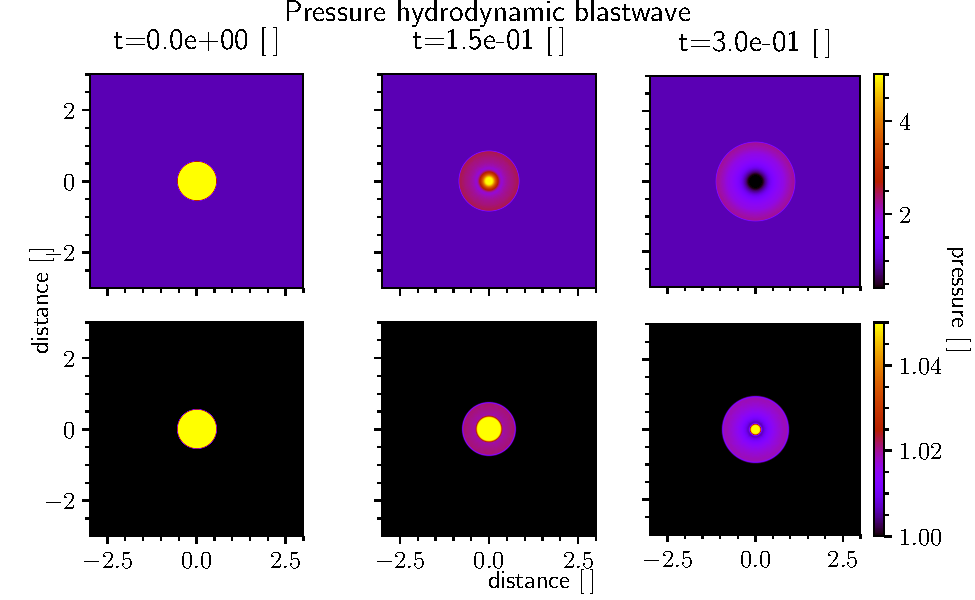
\includegraphics[width=\linewidth]{images/HD-blast-prs-1.pdf}
	\caption{Pressure profile for a blastwave in an ideal fluid at different times. The top row start with the larger pressure difference of $5/1$, the bottom row is the blastwave with smaller pressure difference of $1.5/1$.}
	\label{fig:HD-blast-short}
\end{figure}

\begin{figure}[h]
	%\hspace{-1cm}
	\centering
	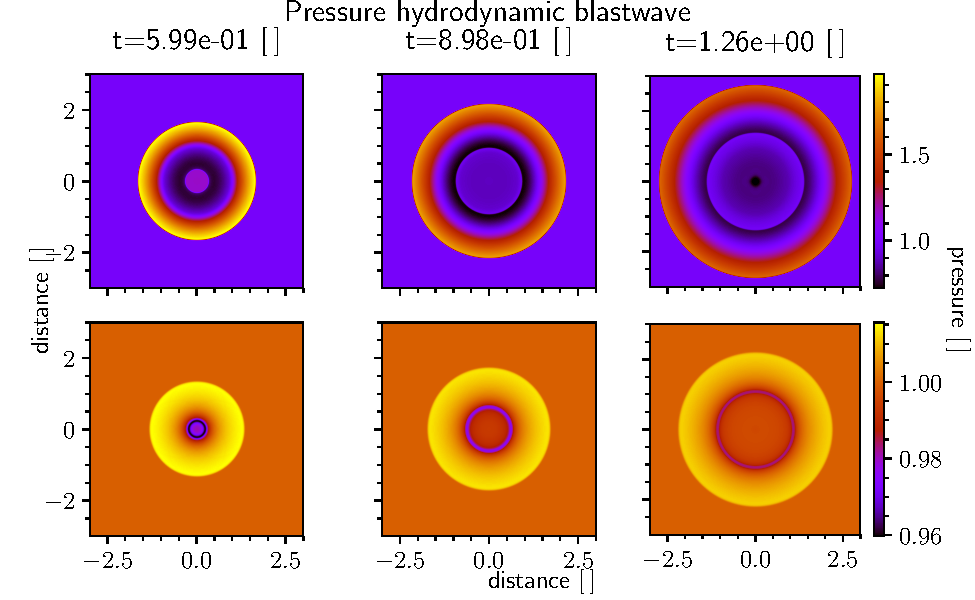
\includegraphics[width=\linewidth]{images/HD-blast-prs-2.pdf}
	\caption{Pressure profile for a blastwave in an ideal fluid at larger timescales. Initial conditions for each row are the same as in \autoref{fig:HD-blast-short}.}
	\label{fig:HD-blast-long}
\end{figure}

\begin{figure}[h]
	%\hspace{-1cm}
	\centering
	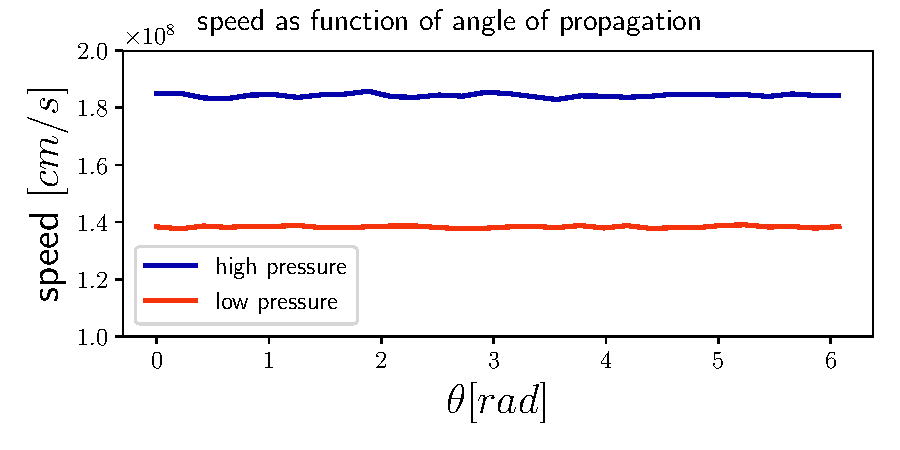
\includegraphics[width=\linewidth]{images/speed-angle-hd.pdf}
	\caption{The wave speed as a function of the angle between the $x$-axis and the line connecting a point on the wave-front with the center of the domain. The wavespeed is calculated from the simulation data.}
	\label{fig:speed-angle-hd}
\end{figure}

\begin{figure}[H]
	%\hspace{-1cm}
	\centering
	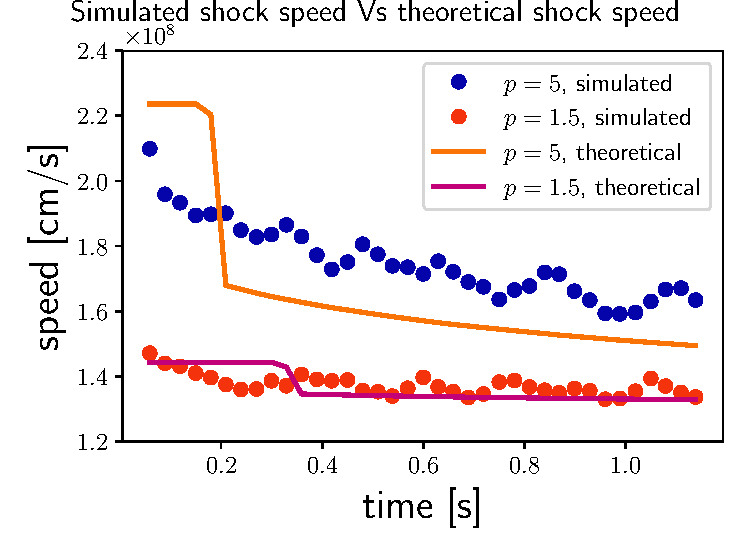
\includegraphics[width=\linewidth]{images/speed-time-hd.pdf}
	\caption{the speed of the wave as a function of time, along the $x$-axis. The dots represent the speed calculated from the simulation data by deriving the function $x(t)$ that represents the position of the wave front. The lines represent the theoretical shock speed in a Riemann-problem with as high pressure the highest pressure in the domain, and low pressure $1$.}
	\label{fig:speed-time-hd}
\end{figure}


test
